\section*{Preface}
This chapter is about discovering a material which achieved one of the highest specific capacities for non-aqueous aluminium-ion batteries! Boron nitride was tested as a cathode material and it showed a very high discharge capacity (>250 mAh g$^{-1}$). However, it turned out that boric anhydride (\ce{B2O3}), which was an impurity in hexagonal boron nitride (hBN), was the active material. Pure \ce{B2O3} was tested as a cathode material, the battery produced a similar discharge capacity of >250 mAh g$^{-1}$.   

\begin{figure}[tbh!]
\centering
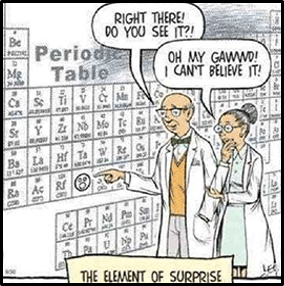
\includegraphics[width=0.5\textwidth]{Figures/BOhBN/ah}
\end{figure}

\newpage
\chapter{Boron nitride/boron oxide as cathodes for rechargeable AIBs} 
\label{BOhBN} 

\section{Theory and background}
Graphite has been extensively used as a cathode in AIBs due to its high conductivity and a layered structure. Graphite and hexagonal boron nitride (hBN) are two prominent members of layered materials possessing a hexagonal lattice structure \cite{hod_graphite_2012}. Graphite has non-polar homonuclear C-C intralayer bonds, hBN presents highly polar B-N bonds resulting in different optimal stacking modes of the two materials in the bulk form. Furthermore, the static polarizabilities of the constituent atoms considerably differ from each other, suggesting large differences in the dispersive component of the interlayer bonding. Despite these major differences, both materials present practically identical interlayer distances, Figure \ref{Figures/BOhBN:grpBNcomp}. hBN is popularly known as "white graphene" \cite{song_large_2010, zeng_white_2010}. Structurally, a single layer of hBN is very similar to a graphene sheet having a hexagonal backbone where each couple of bonded carbon atoms is replaced by a boron nitride pair, making the two materials isoelectronic. Nevertheless, due to the electronegativity differences between the boron and the nitrogen atoms, the $\pi$ electrons tend to localize around the nitrogen atomic centers, thus forming an insulating material. The nature of bonding between nitrogen and boron differs from the carbon-carbon bonds found in graphite. hBN possesses coordinate bonds resulting from donation of \ce{e-} pair from nitrogen into empty p-orbital of a neighbouring B atom. Each N atom develops a partial positive charge and each B develops a partial negative charge. The partial ionic character of BN bonding makes it a semi-conductor as opposed to a conductor like graphite. 

\section{Results and discussion}

\begin{figure}[tbh!]
\centering
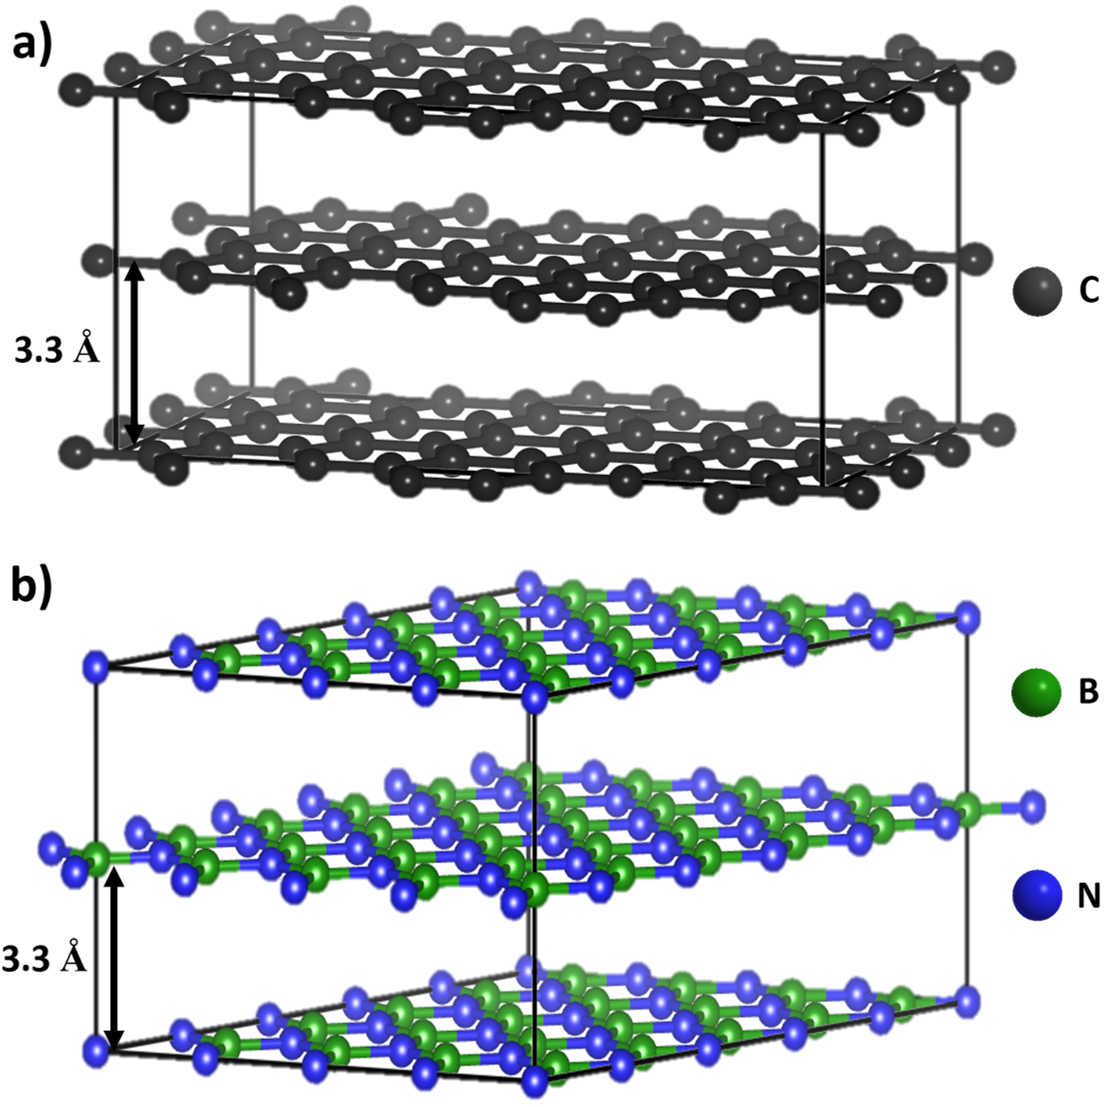
\includegraphics[width=\textwidth]{Figures/BOhBN/grpBNcomp}
\caption{Honeycomb lattice of a) natural graphite and b) hexagonal boron nitride. They have similar interlayer distance of 3.3\AA.}
\label{Figures/BOhBN:grpBNcomp}
\end{figure}

For all the above mentioned reasons, we tested hBN as a cathode for AIBs. To save cost, hBN was retrieved from VUW's chemical stores. An aluminium-ion cell was assembled using hBN as the cathode and preliminary electrochemical tests were performed, Figure \ref{Figures/BOhBN:hBNiniCDC}. hBN showed very high specific capacities for the first 30 cycles. It recorded a capacity of 270 mAh g$^{-1}$ which decreased to 100 mAh g$^{-1}$ at a discharge potential of 0.6 V. In spite of having a very similar to graphite and not being as conductive, this value was almost 3 times than that of graphite (inset, Figure \ref{Figures/BOhBN:hBNiniCDC}). Repeated experiments from a single batch of hBN cathodes gave us similar results, Figure \ref{Figures/appendix:hBNrepeat}. In expectation of better results, we bought a new bottle of hBN (Sigma Aldrich, 98\%, $\approx$1 $\mu$m in size). New batch of electrodes were made but surprisingly the cells did not record a capacity, which was anywhere near the previous cells, Figure \ref{Figures/BOhBN:hBNCDCCE}. We made many more batches of cathodes, yet the cells did not yield similar numbers after several reruns (Figure \ref{Figures/appendix:hBNmultiattempts}! It was important to examine the difference between the two hBNs. We analysed the XPS spectra of hBN from our chemical stores as shown in Figure \ref{Figures/BOhBN:oldhBNXPS}. The spectra compared pristine, charged and discharged electrodes after they were washed with dry ethanol to get rid of any residual electrolyte. Pristine cathode observed the characteristic 1s peak of BN at 192 eV (. However, Gaussian peak fitting revealed presence of another peak at 193.5 eV , which corresponded to \ce{B2O3}. 
\begin{figure}[tbh!]
\centering
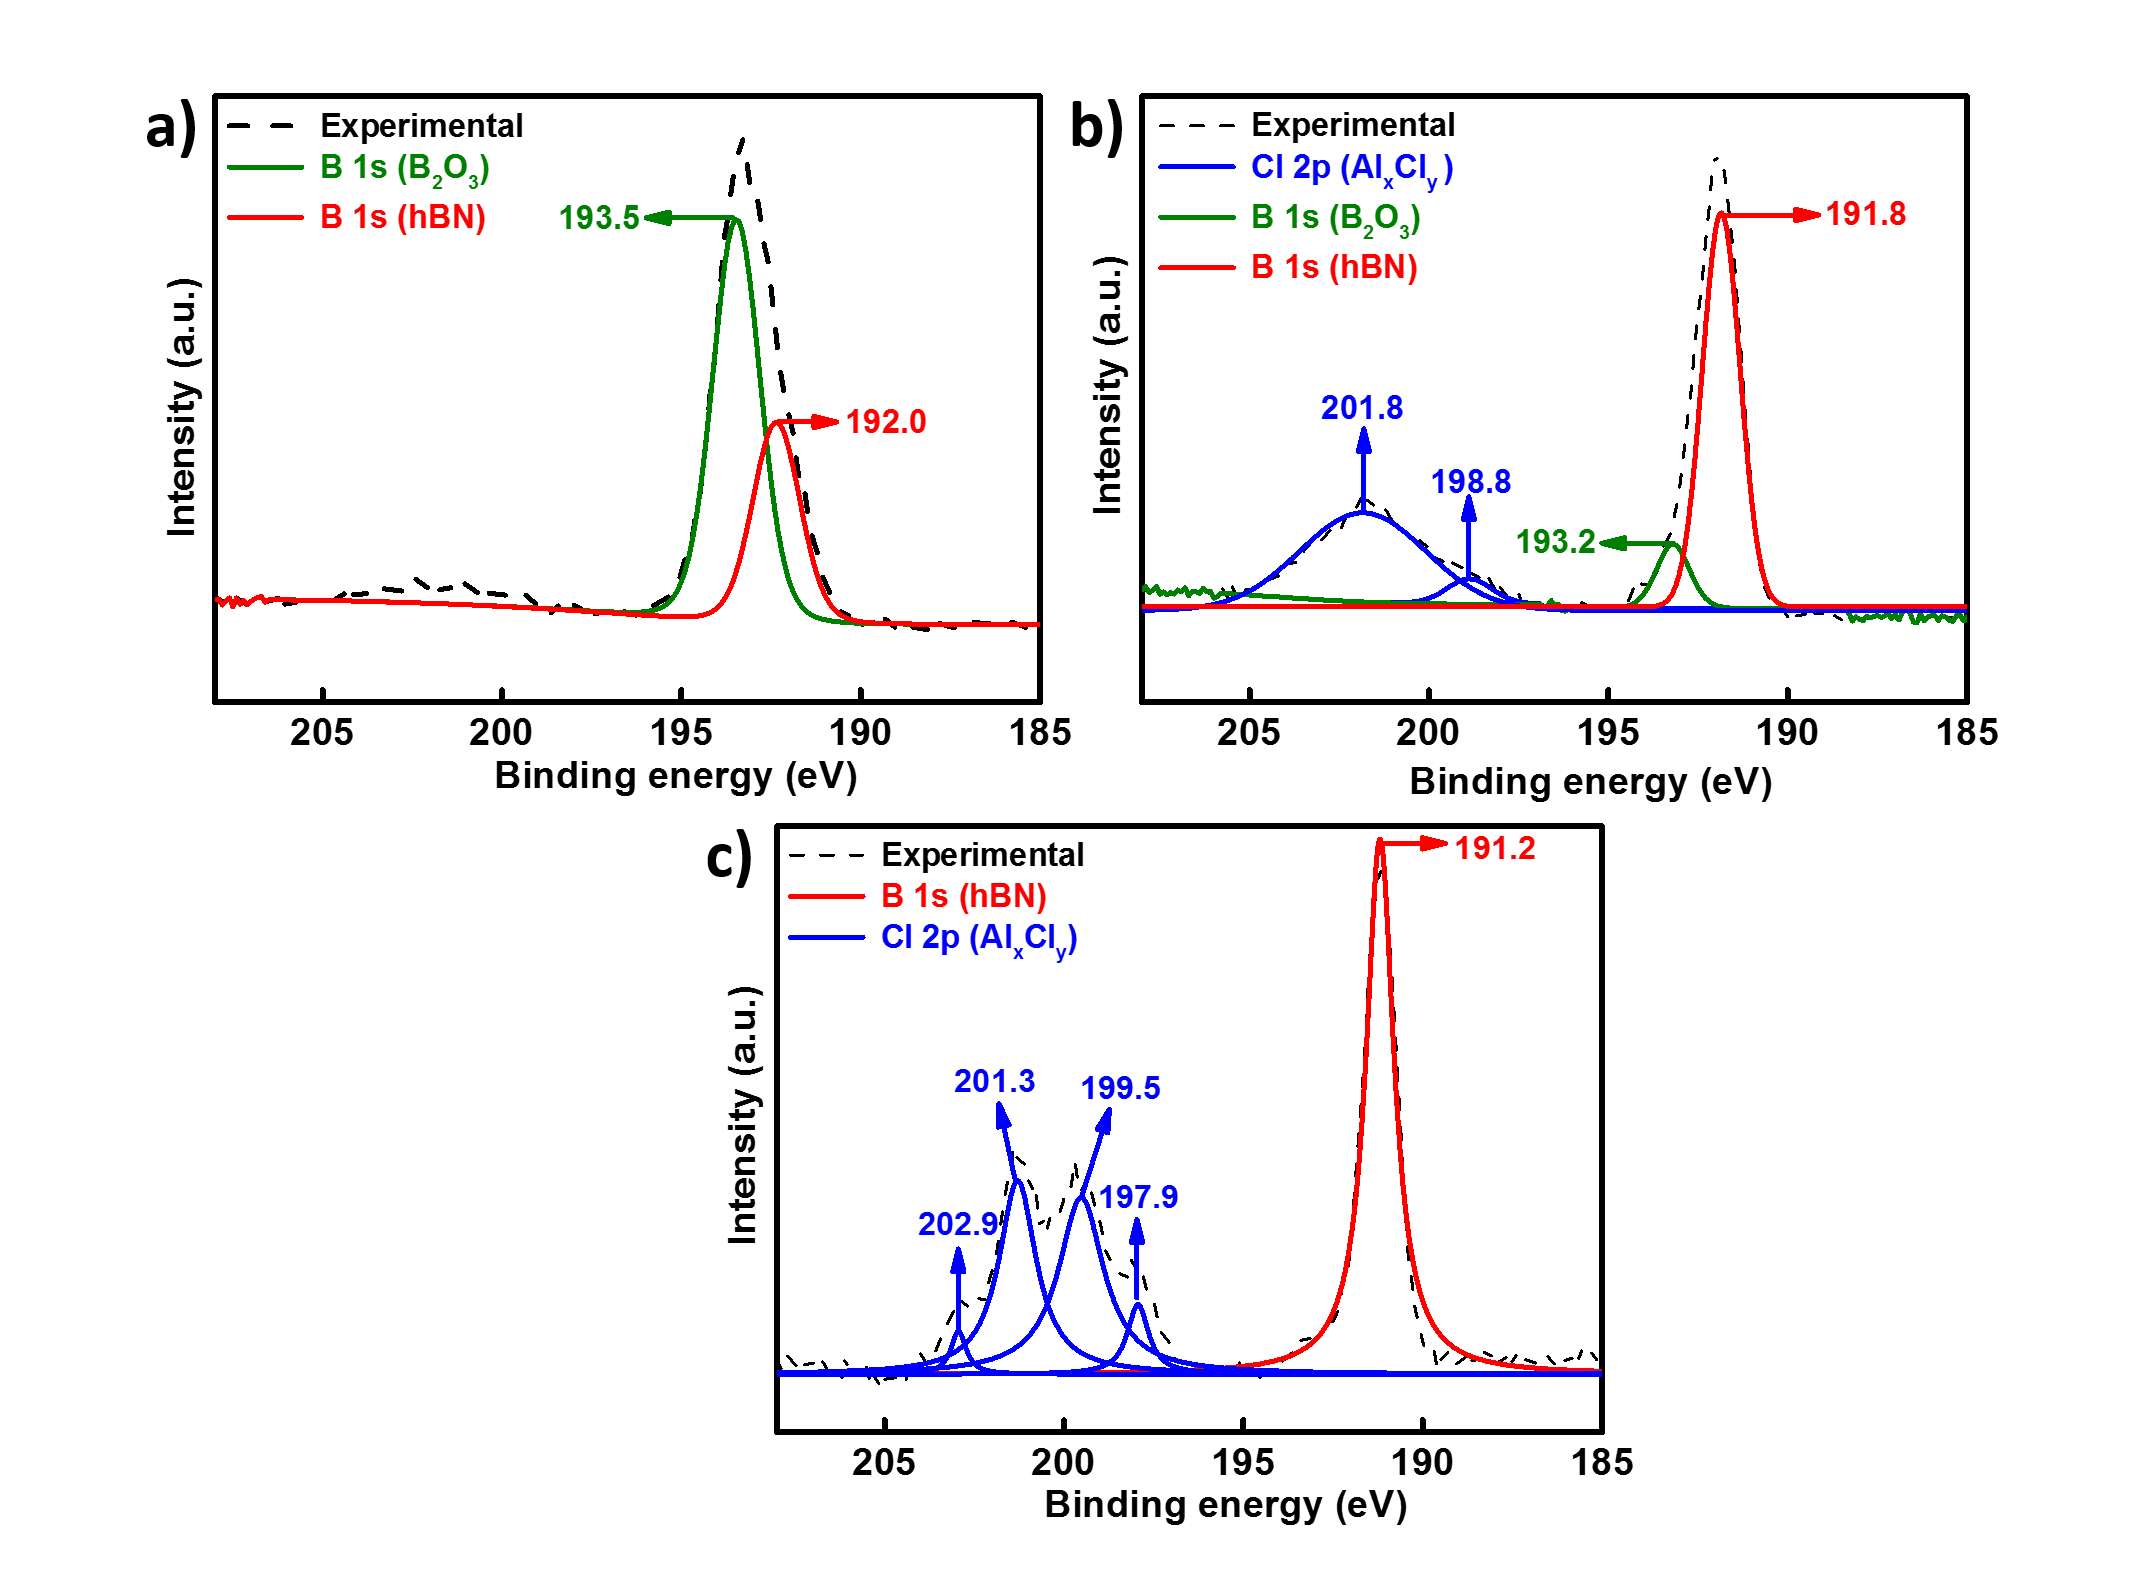
\includegraphics[width=\textwidth]{Figures/BOhBN/oldhBNXPS}
\caption{XPS spectra of a a) pristine, b) charged and c) discharges old hBN cathodes after 30 cycles.}
\label{Figures/BOhBN:oldhBNXPS}
\end{figure}
 \begin{figure}[tbh!]
\centering
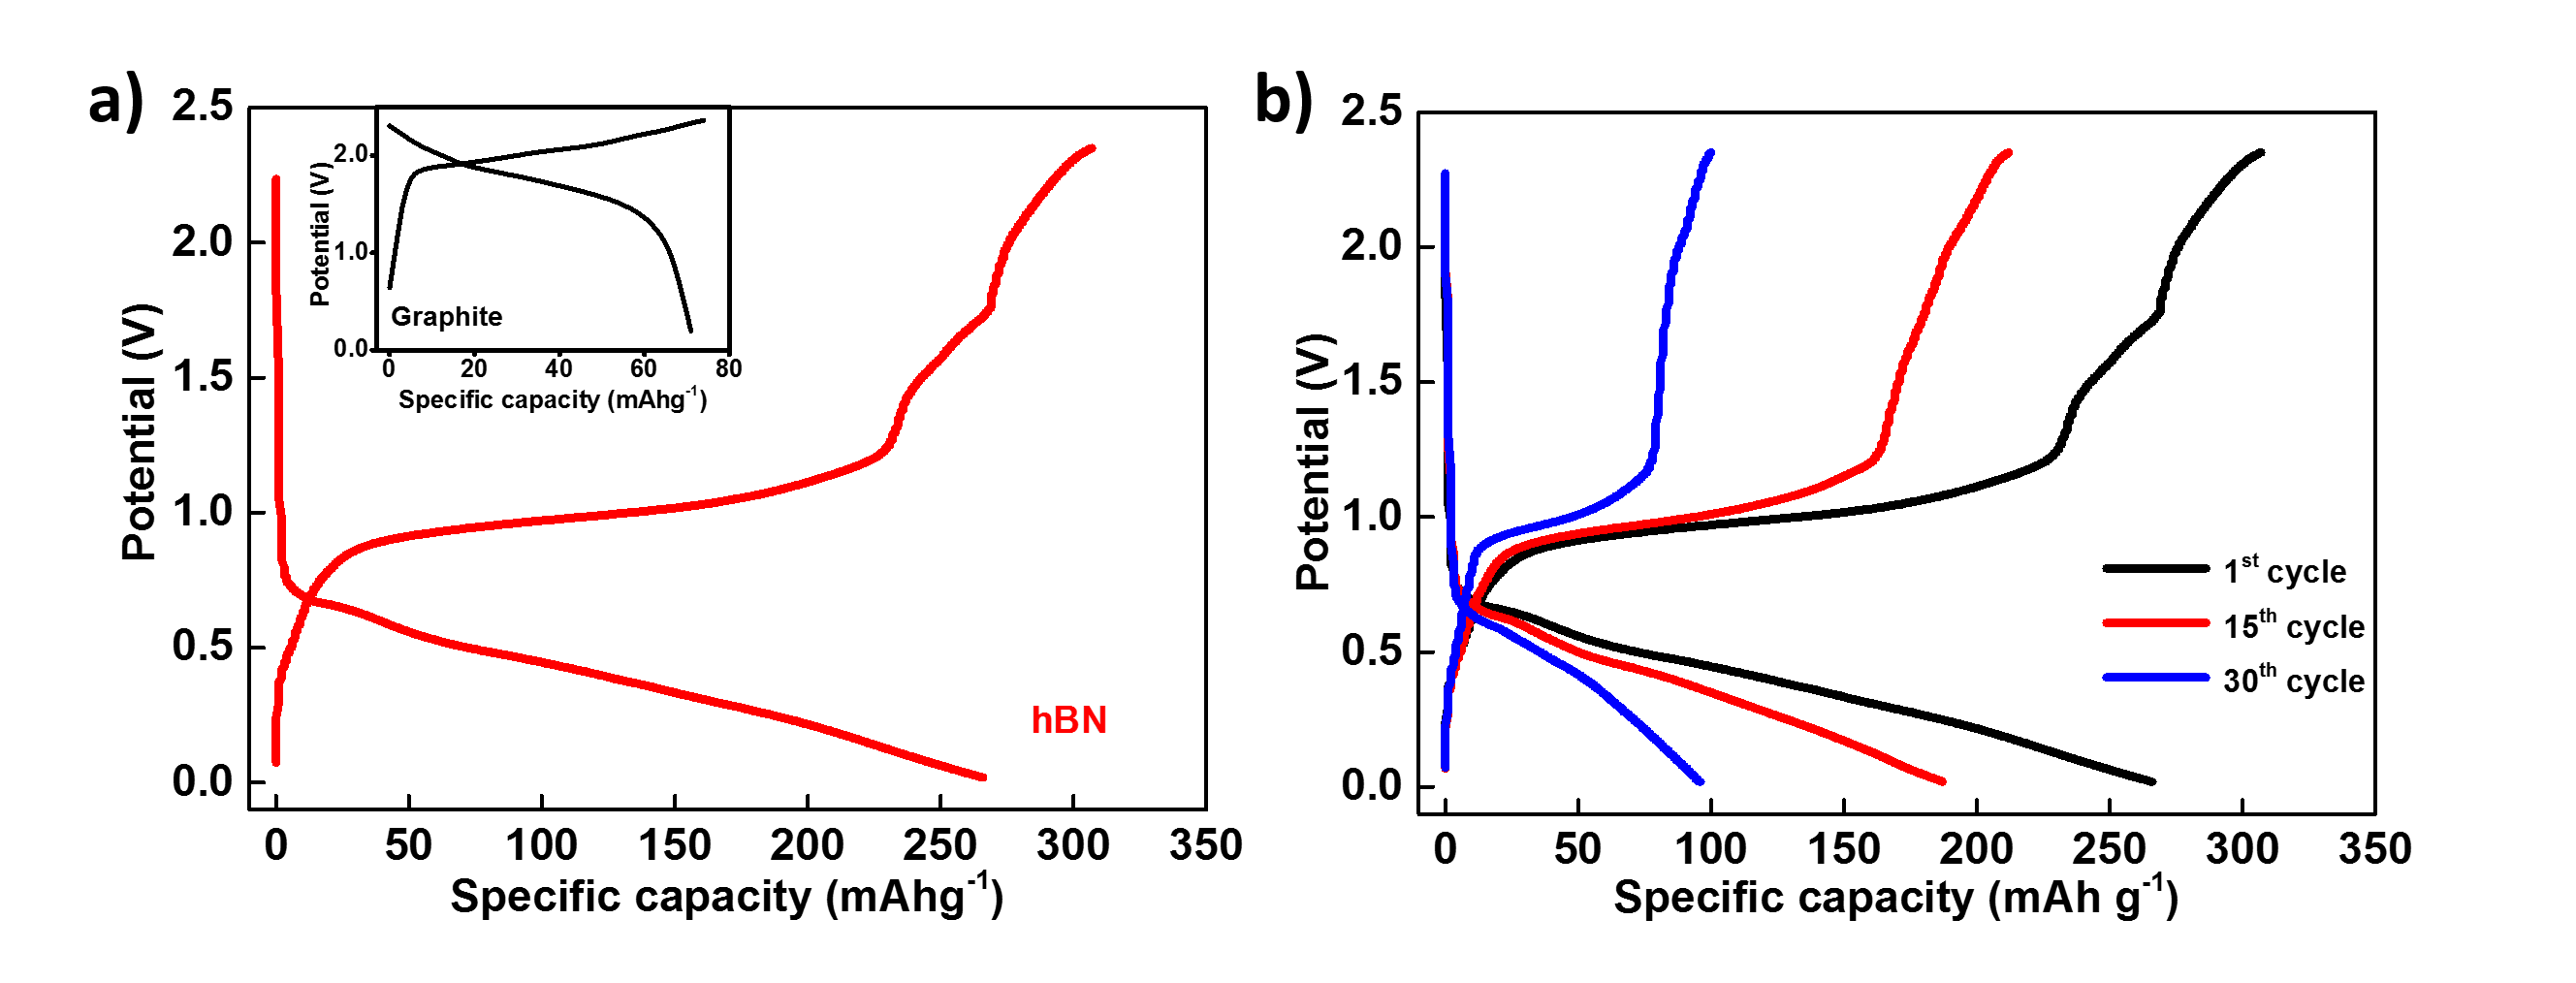
\includegraphics[width=\textwidth]{Figures/BOhBN/hBNiniCDC}
\caption{a) Galvanostatic cycles of an Al/hBN, using old hBN from the stores, at a current density of 50 mA g$^{-1}$ compared with natural graphite (inset). b) Capacity fading of Al/hBN cell recorded for 30 cycles at a current rate of 50 mA g$^{-1}$.}
\label{Figures/BOhBN:hBNiniCDC}
\end{figure}
\begin{figure}[tbh!]
\centering
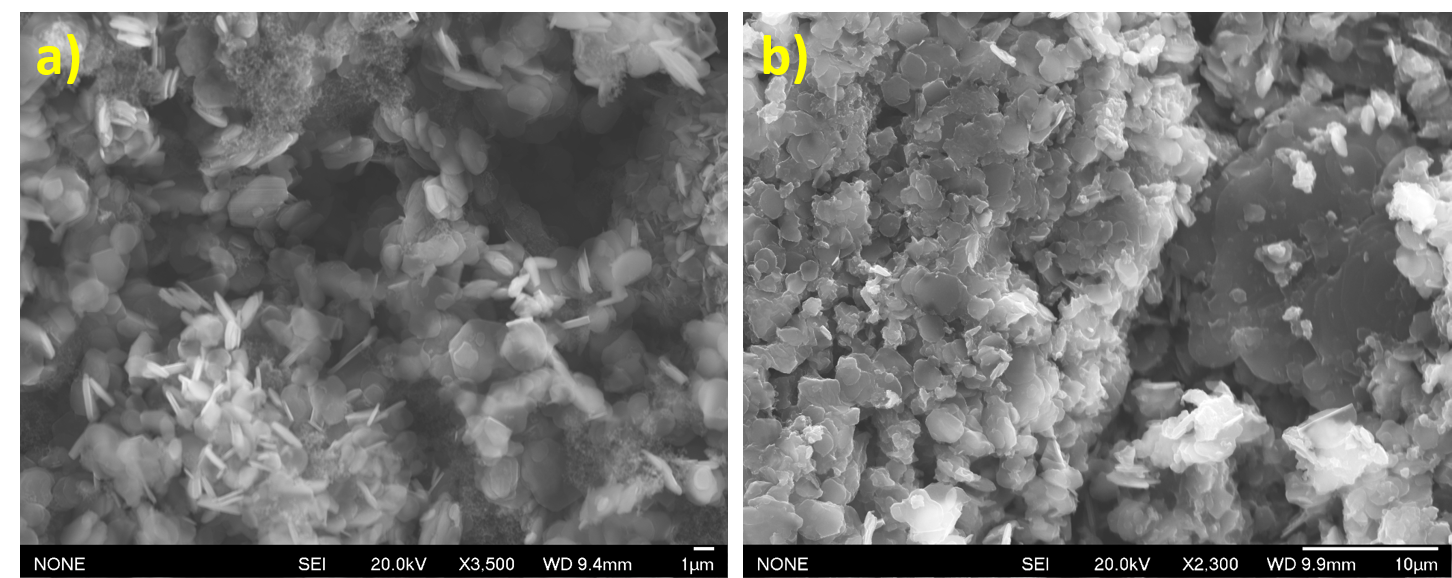
\includegraphics[width=\textwidth]{Figures/BOhBN/hBNSEM}
\caption{SEM images of a pristine hBN cathode using old hBN at different magnifications. The hexagonal structure of boron nitride can be seen clearly.}
\label{Figures/BOhBN:hBNSEM}
\end{figure}
\begin{figure}[tbh!]
\centering
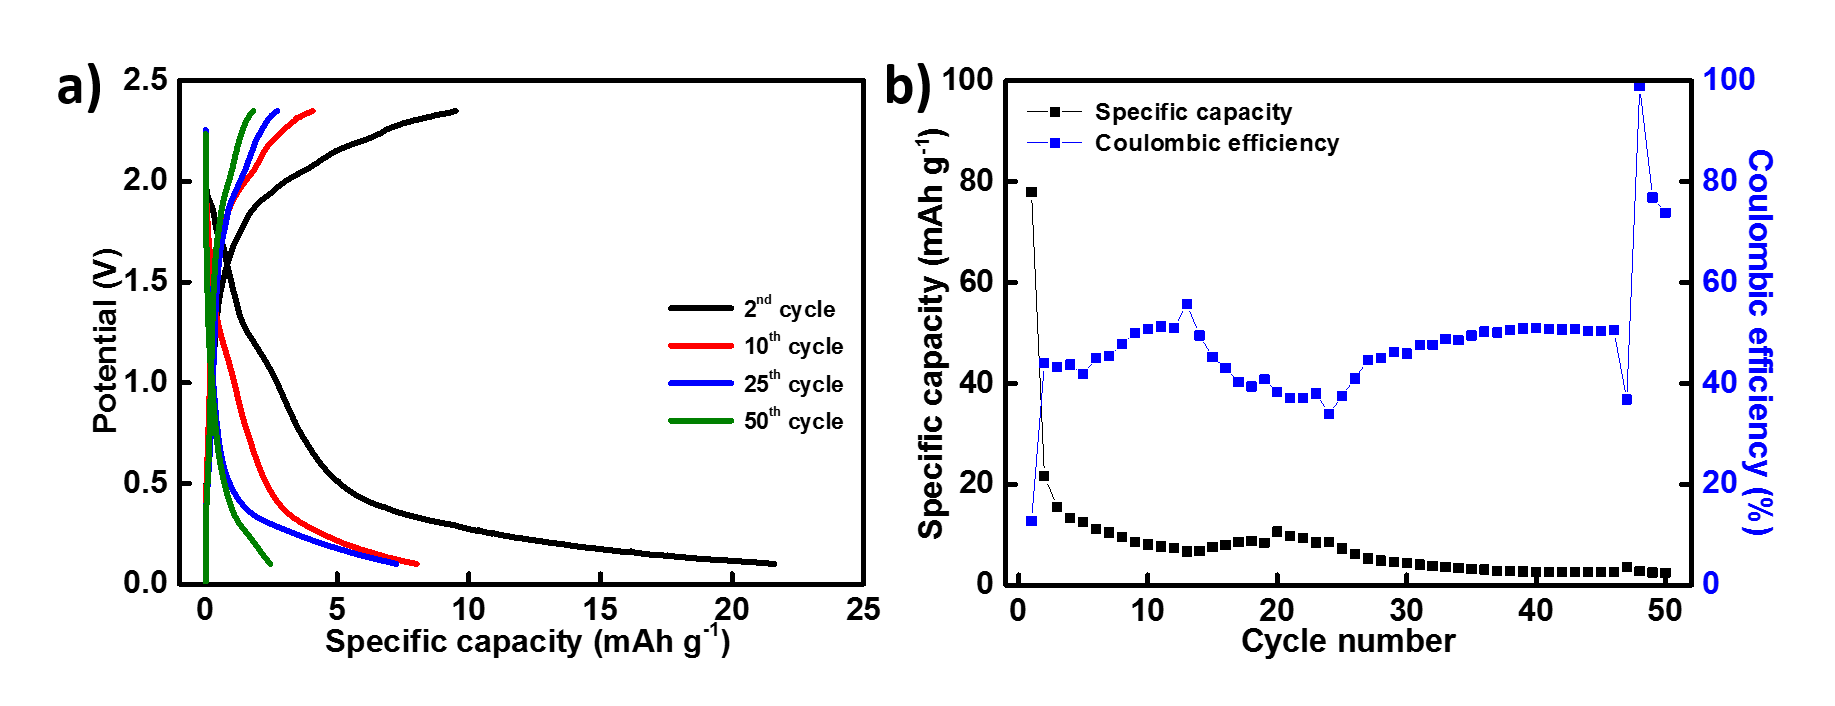
\includegraphics[width=\textwidth]{Figures/BOhBN/BNNSCDCCE}
\caption{a) Galvanostatic cycles of an Al/hBN at a current rate of 50 mA g$^{-1}$ in a two-electrode setup, b) The cell seems to become inactive after rapid capacity decay (capacity reaches zero after 50 cycles with a very poor cell efficiency $\approx$ 55\% at a current rate of 50 mA g$^{-1}$.}
\label{Figures/BOhBN:hBNCDCCE}
\end{figure}
\begin{figure}[tbh!]
\centering
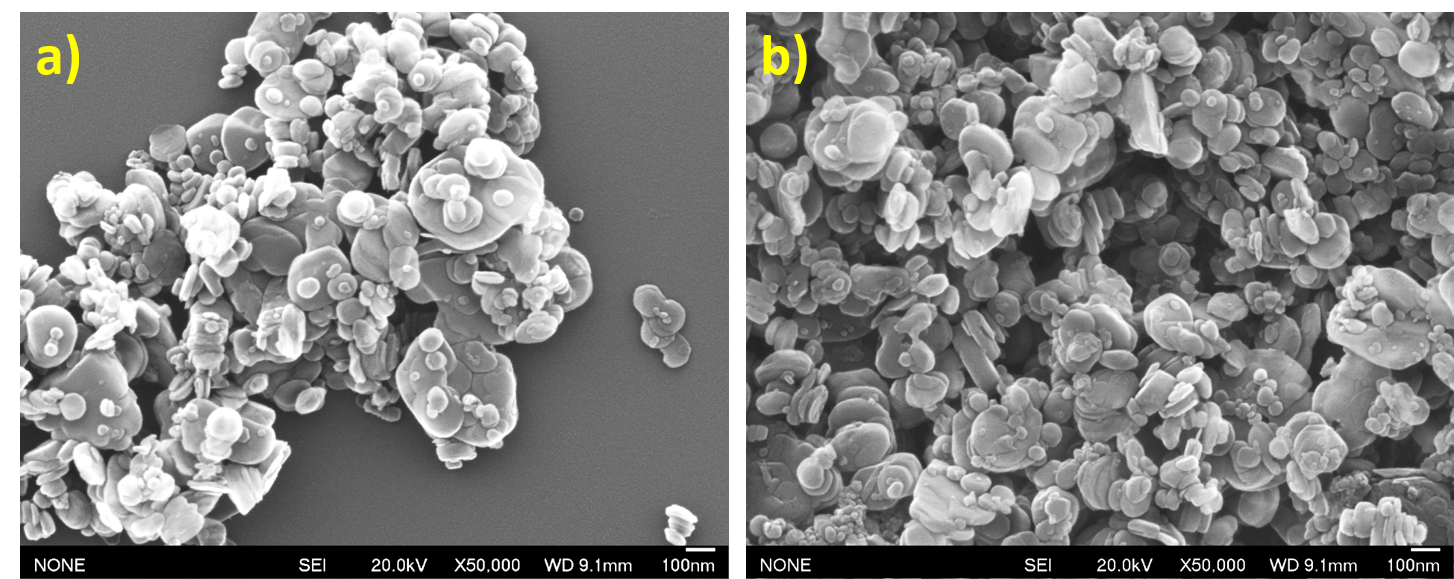
\includegraphics[width=\textwidth]{Figures/BOhBN/BNNSSEM}
\caption{a) Coulombic efficiency recorded for 1600 cycles of an Al/hBN pouch cell assembled in IKTS, Germany.}
\label{Figures/BOhBN:BNNSSEM}
\end{figure}
\begin{figure}[tbh!]
\centering
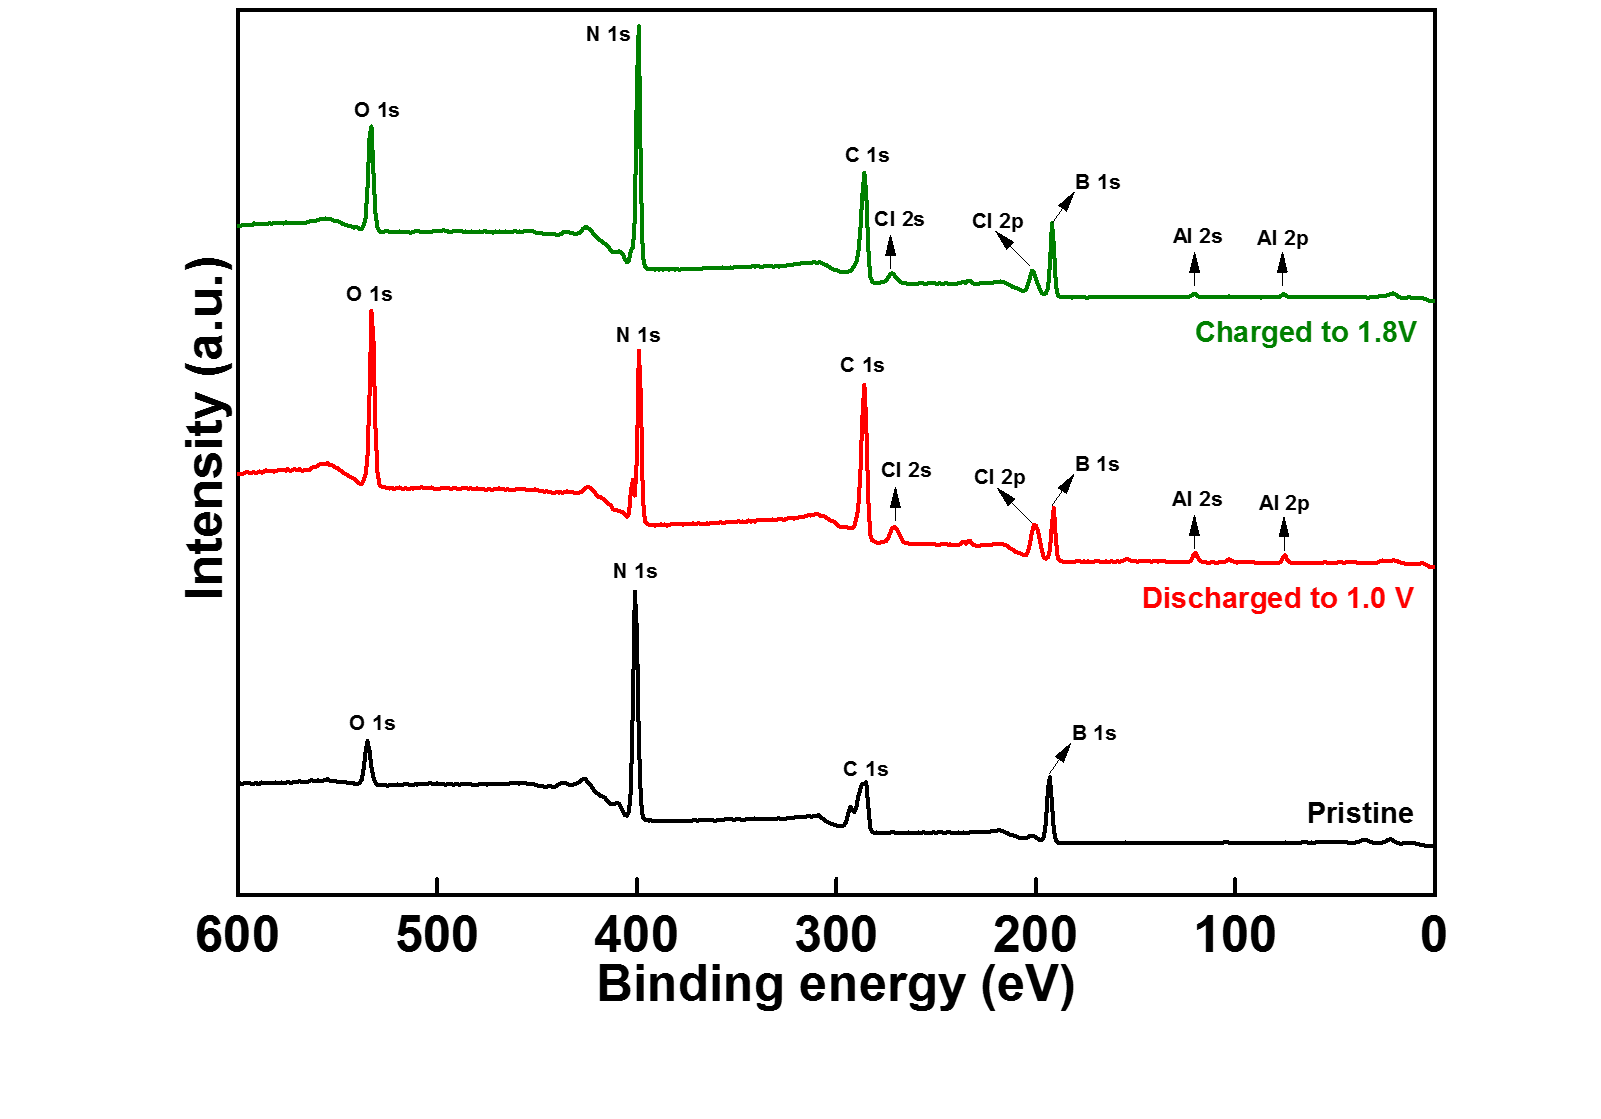
\includegraphics[width=\textwidth]{Figures/BOhBN/hBNXPS}
\caption{a) Coulombic efficiency recorded for 1600 cycles of an Al/hBN pouch cell assembled in IKTS, Germany.}
\label{Figures/BOhBN:hBNXPS}
\end{figure}
\section{Experimental methods}
Same as described in previous chapters.
\section{Conclusion and future outlook}
